\section{Application of probabilistic catalogs for population studies}
\lb{sec:dNdS}



\begin{figure}[h]
%\hspace*{-1cm}
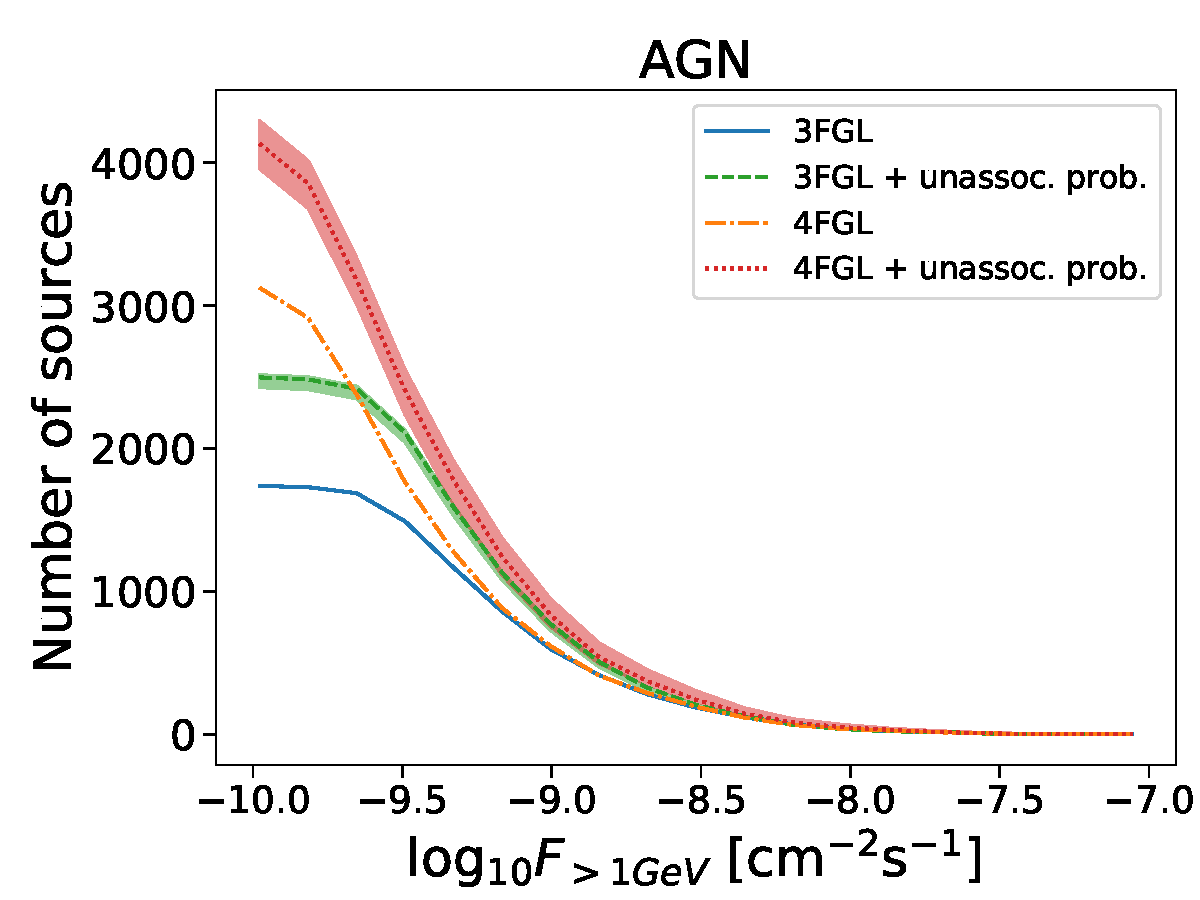
\includegraphics[width=0.4\textwidth]{plots/logN_logS_AGN.pdf}
%\hspace*{-1cm}
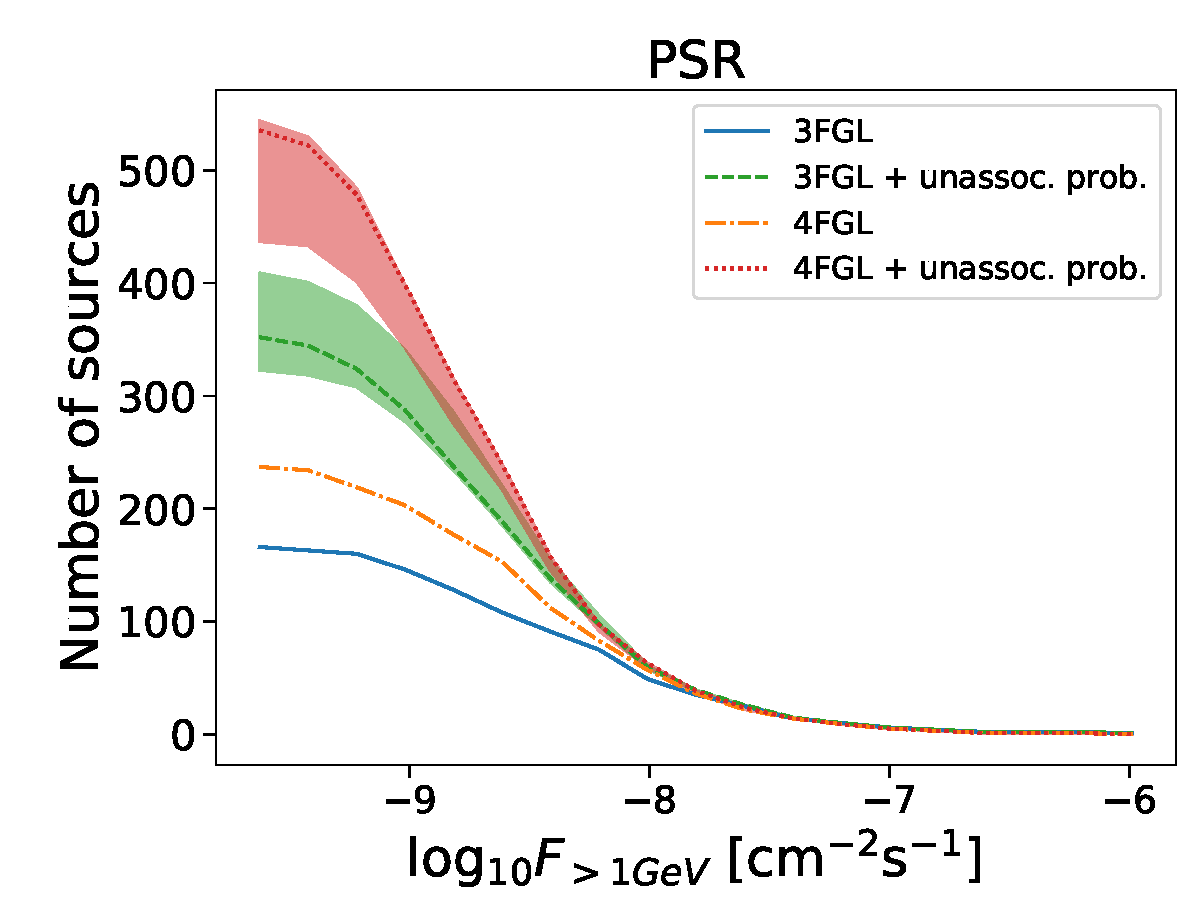
\includegraphics[width=0.4\textwidth]{plots/logN_logS_PSR.pdf}
\caption{Log N - log S.}  
\label{fig:logN_logS}
\end{figure}




\begin{figure}[h]
%\hspace*{-1cm}
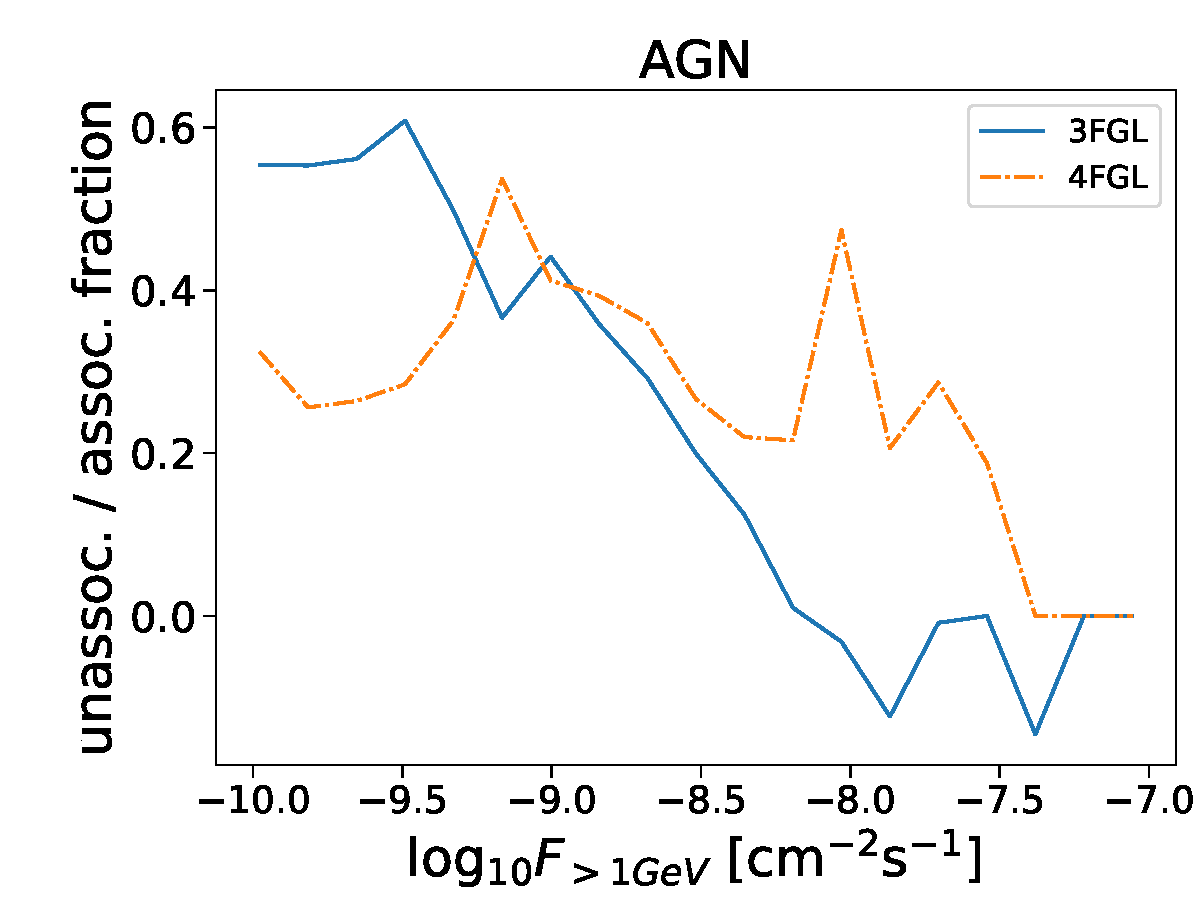
\includegraphics[width=0.4\textwidth]{plots/logN_logS_diff_AGN.pdf}
%\hspace*{-1cm}
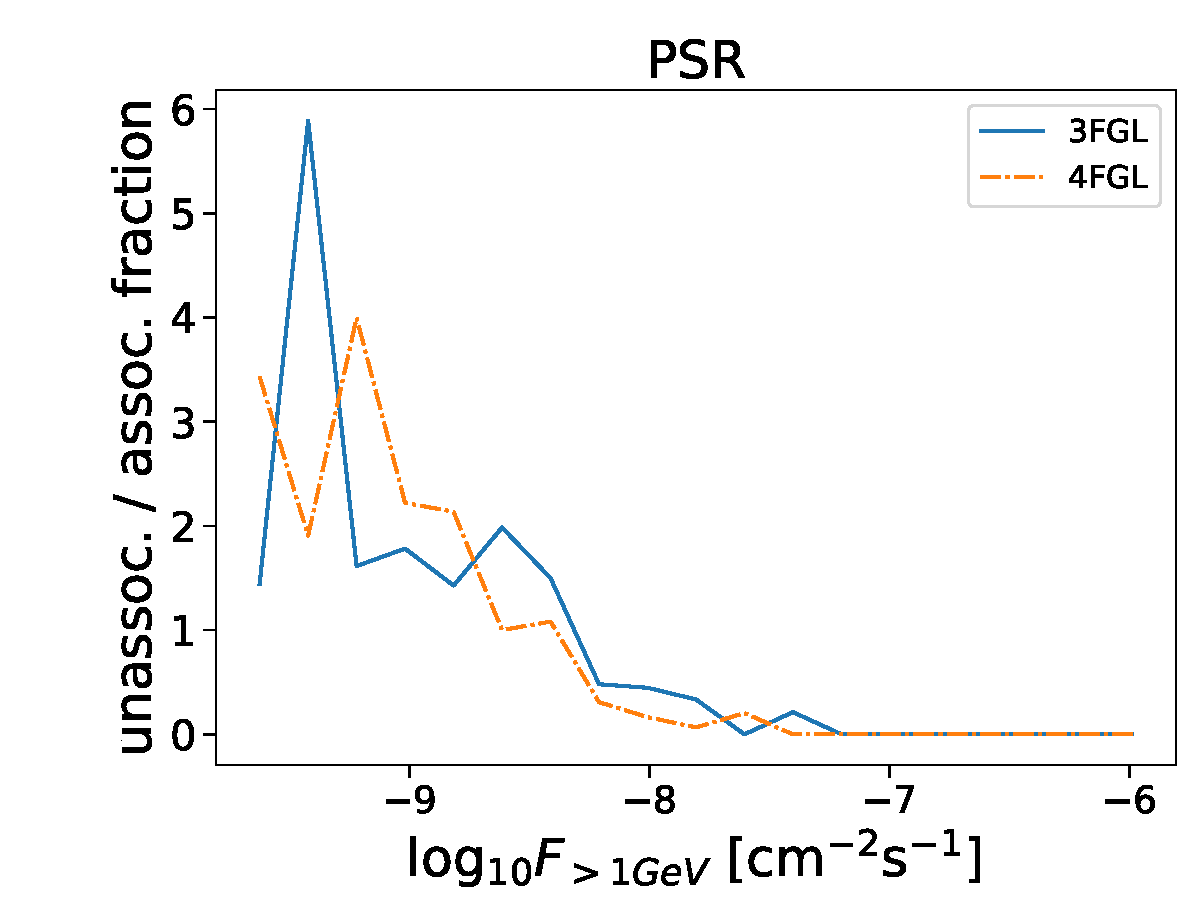
\includegraphics[width=0.4\textwidth]{plots/logN_logS_diff_PSR.pdf}
\caption{Fraction of unassociated sources relative to associated ones.}  
\label{fig:unass_vs_ass_frac}
\end{figure}



In this Section we show how probabilistic catalogs can be used, for instance, for population studies,
which can be used, for instance, to determine the contribution of unresolved point sources to isotropic gamma-ray emission.
Understanding the origin of the isotropic gamma-ray emission is important for placing strong constraints
on dark matter annihilation into gamma rays or evaporation of primordial black holes
as well as constraining the origin of astrophysical high energy neutrino flux.

In Figure \ref{fig:logN_logS} we show the cumulative number of AGNs and pulsars with flux above 1 GeV larger than the
value on the x-axis.
We plot the number of associated sources using solid (3FGL) and dash-dotted (4FGL) lines.
We also add unassociated sources weighted by AGN or PSR probabilities in order to estimate the total number of AGNs and pulsars
among the detected sources.
Dashed and dotted lines show the contribution of unassociated sources in 3FGL and 4FGL respectively using LR algorithm.
The bands show the envelop for the predicted number of sources using all four selected ML algorithms.
The predictions for the number of AGNs and pulsars among the unassociated sources are corrected by the presence of other sources (neither AGNs nor pulsars) in the following way.
We assume that the fractional contribution of other sources is the same for associated and unassociated sources in the different flux bands used in Figure \ref{fig:logN_logS}.
In particular, the number of AGNs among unassociated sources in a certain flux band $\Delta F$ is estimated as
\be
n_{\rm AGN} = \sum_{i \in \rm unassoc.} p^i_{\rm AGN}\,\, - \sum_{i \in \rm assoc.\,other} p^i_{\rm AGN} \cdot \frac{n_{\rm unassoc.}}{n_{\rm assoc.}}
\ee
where all probabilities and the numbers of sources are computed for sources with flux inside $\Delta F$.
The first term is the sum of AGN-like probabilities among the unassociated sources,
while the second term is the sum of AGN-like probabilities among associated ``other'' sources rescaled by the total number
of unassociated and associated sources in this flux band.
The number of pulsars among the unassociated sources is calculated analogously.

